\clearpage\newpage
\subsection{Flowcharts}

The processes of the app are optimized to be notably simple because it has to be easy-to-use. Most of the common actions are 1 to 3 clicks away from the dashboard. 


\subsubsection*{Add subject}

This process consists of adding subjects to the dashboard. It is precisely represented in the \textbf{Figure \ref{flowchart-add-subject}}. Check it out carefully to understand all the paths.

Although it may look complex, usually, it's stunningly simple. With 4 interactions a subject can be added:
\begin{enumerate}
    \item Click the add button in the dashboard. To open the search screen.
    \item Type the name of the subject. The search field is focused automatically, so the user doesn't have to click it.
    \item Click the desired search result's checkbox. % switching from \inlineicon{button-search-gray.png} to \inlineicon{button-search-green.png}.
    \item Click the add button in the search screen.
\end{enumerate}

\noindent
The process becomes difficult when the subject is not already in the database. When that happens the user has to create the subject. There's also the possibility of editing a subject before adding it, but it's totally optional.

% \begin{itemize}
%     \item Google or receive url from a friend
%     \item See tutorial, + button animation
%     \item Search
%     \begin{enumerate}[label=\Alph*]
%         \item Finds subject and continues
%         \item Doesn't find the subject closes the app
%         \item Doesn't find the subject, and tries to create it
%         \begin{enumerate}[label=\Alph*]
%             \item Manages to create it
%             \item Doesn't understand it and closes the app
%         \end{enumerate}
%     \end{enumerate}
%     \item fills the grades
%     \begin{enumerate}[label=\Alph*]
%         \item Understands the meaning of the gray numbers
%         \item Doesn't understand it and just uses the app to store the grades.
%     \end{enumerate}
% \end{itemize}

\clearpage\newpage
\vfill
\begin{figure}[ht!]
    \center
    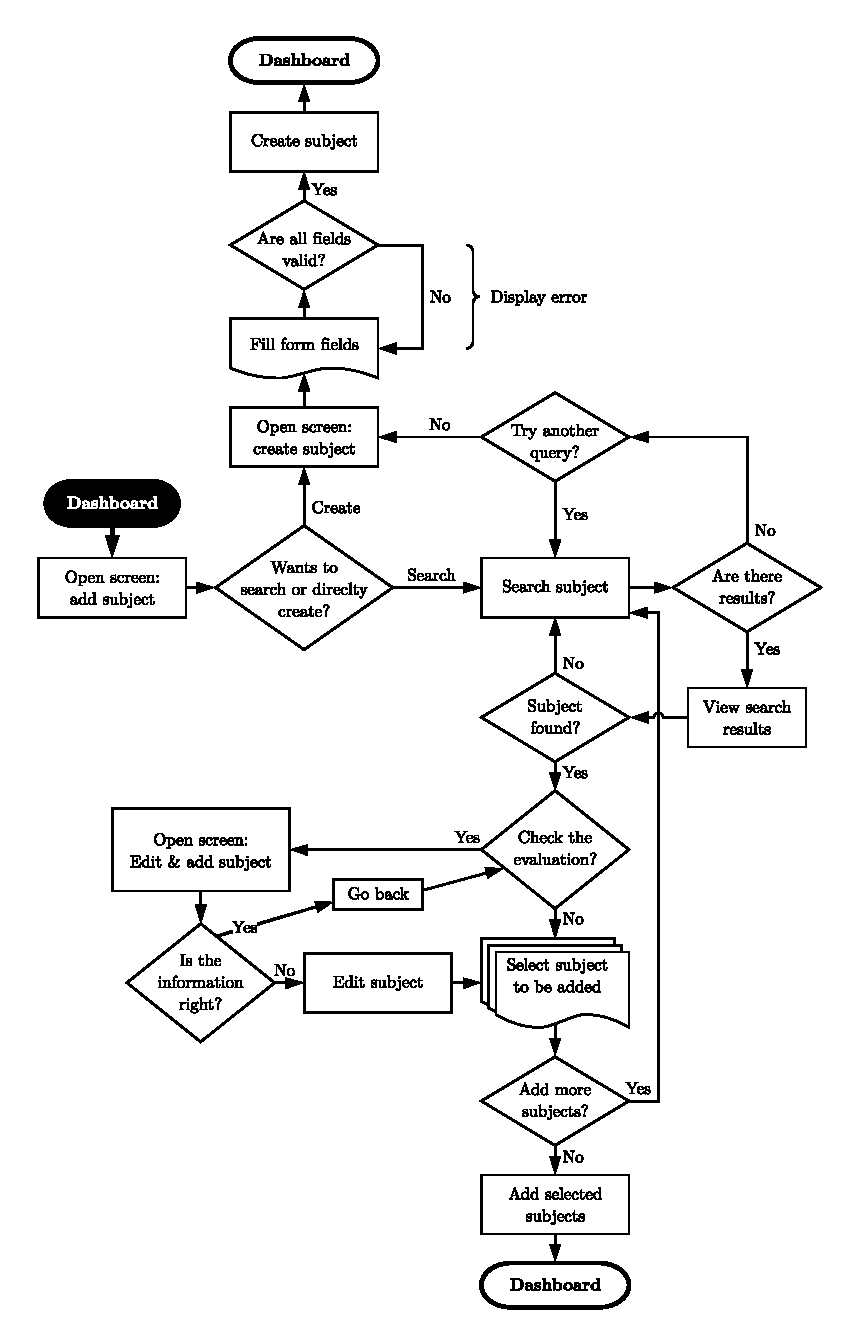
\includegraphics[height=\textheight-1cm]{media/diagrams/flowchart-add-subject.pdf}
    % [height=\textheight-2.15cm]  with a \subsubsection on the same page
    \caption{Flowchart of adding a subject}
    \label{flowchart-add-subject}
\end{figure}
\vfill

\clearpage\newpage
\subsubsection*{More relevant processes}

\vfill
\begin{figure}[ht!]
    \vspace*{-1.5in}
    
\includegraphics[scale=1]{media/diagrams/flowchart-login.pdf}
    \vspace*{-0.125in}
    \caption{Flowchart of logging-in}
    \label{flowchart-login}
\end{figure}
\vfill
\vspace*{-1.5in}
\begin{figure}[ht!]
    
\includegraphics[scale=1]{media/diagrams/flowchart-logout.pdf}
    \vspace*{-0.125in}
    \caption{Flowchart of logging-out}
    \label{flowchart-logout}
\end{figure}
\vfill
\begin{figure}[ht!]
    \vspace*{-1.5in}
    
\includegraphics[scale=1]{media/diagrams/flowchart-edit-subject.pdf}
    \vspace*{-0.125in}
    \caption{Flowchart of editing a subject card}
    \label{flowchart-edit-subject}
\end{figure}
\vfill
\begin{figure}[ht!]
    \vspace*{-1.5in}
    
\includegraphics[scale=1]{media/diagrams/flowchart-delete-subject.pdf}
    \vspace*{-0.125in}
    \caption{Flowchart of deleting a subject card}
    \label{flowchart-delete-subject}
\end{figure}
\vfill
\begin{figure}[ht!]
    \vspace*{-1.5in}
    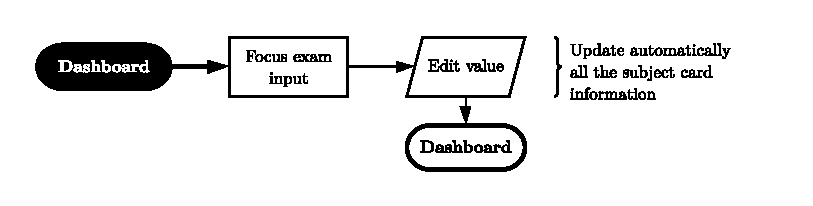
\includegraphics[scale=1]{media/diagrams/flowchart-edit-grade.pdf}
    \vspace*{-0.125in}
    \caption{Flowchart of editing a grade}
    \label{flowchart-edit-grade}
\end{figure}
\vfill
\begin{figure}[ht!]
    \vspace*{-1.5in}
    
\includegraphics[scale=1]{media/diagrams/flowchart-install.pdf}
    \vspace*{-0.125in}
    \caption{Flowchart of the installation}
    \label{flowchart-install}
\end{figure}
\vspace*{-1.5in}
\vfill

% \clearpage\newpage
% \subsubsection{Add subject}

% \begin{figure}[ht!]
%     \center
%     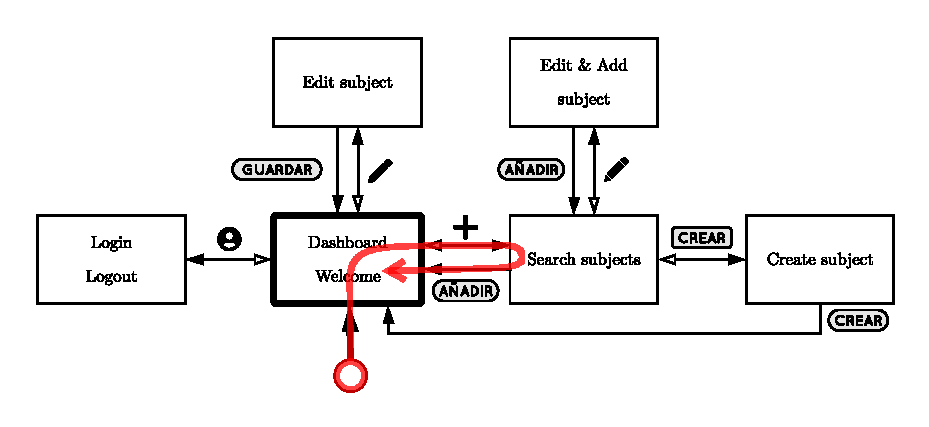
\includegraphics[width=1\columnwidth]{media/diagrams/flow-search.pdf}
%     \caption{Flow search and add subject}
%     \label{fig:flow-search}
% \end{figure}

% \begin{figure}[ht!]
%     \center
%     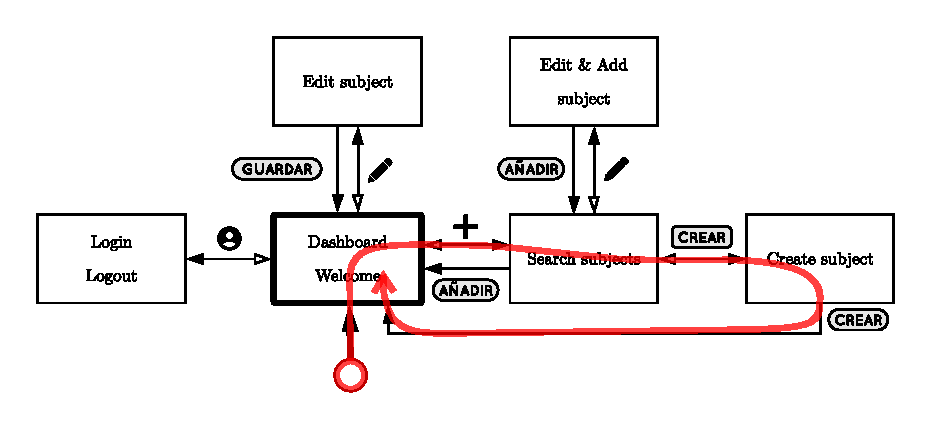
\includegraphics[width=1\columnwidth]{media/diagrams/flow-create.pdf}
%     \caption{Flow create subject}
%     \label{fig:flow-create}
% \end{figure}

% \clearpage\newpage
% \subsubsection{Login}

% \begin{figure}[ht!]
%     \center
%     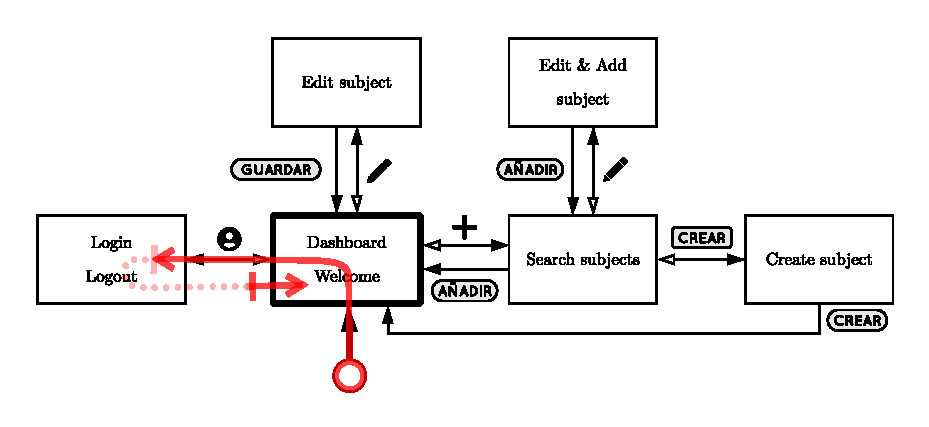
\includegraphics[width=1\columnwidth]{media/diagrams/flow-login.pdf}
%     \caption{Flow login or singing}
%     \label{fig:flow-login}
% \end{figure}

% \clearpage\newpage
% \subsubsection{Install}

% \begin{figure}[ht!]
%     \center
%     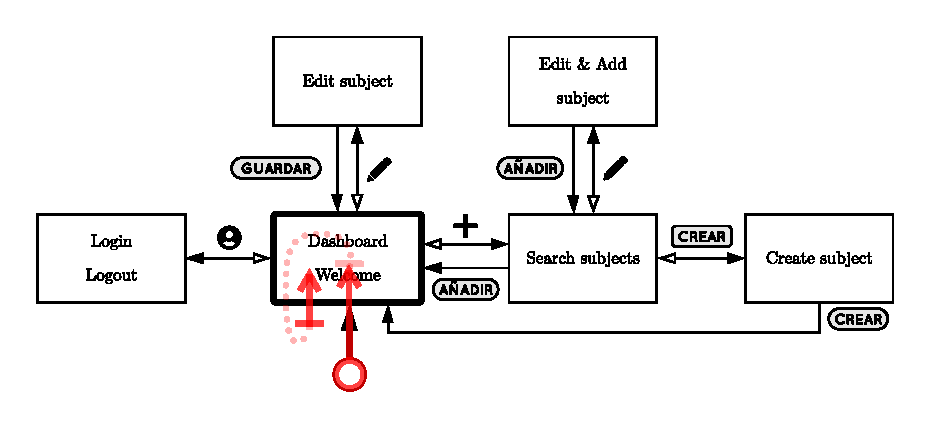
\includegraphics[width=1\columnwidth]{media/diagrams/flow-install.pdf}
%     \caption{Flow install app}
%     \label{fig:flow-install}
% \end{figure}

